\TUsection{Java PathFinder}
\label{sec:jpf}

% (Definition of JPF) (verification, analysis and testing environment for Java, called Java PathFinder (JPF)) (JPF is a highly customizable execution environment for verification of Java™ bytecode programs)

% (Java, Mention and reference it) THE Java® programming language is a general-purpose, concurrent, class-based, object-oriented language. It is designed to be simple enough that many programmers can achieve fluency in the language. The Java programming language is strongly and statically typed. This specification clearly distinguishes between the compile-time errors that can and must be detected at compile time, and those that occur at run time.

%(JPF Motivation Why analyze code and in particular Java) We believe it is an attractive idea to develop a verification environment for Java for three reasons. First, Java is a modern language featuring important concepts such as object-orientation and multi-threading within one language. Second, Java is simple, for example compared to C++. Third, Java is compiled into bytecode, and hence, the analysis can be done at the bytecode level. This implies that such a tool can be applied to any language that can be translated into bytecode.

%(Why Java --- It is well known that concurrent programs are non-trivial to construct, and with Java essen- tially giving the capability for anyone to write concurrent programs, we believe, a model checker for Java might have a bright future. In fact, one area where we believe it can have an immediate impact is in environments where Java is taught. Also because it is widely used.)

%(Maybe not necessary but valuable to explain native calls --- The JVMJPF supports all Java bytecodes, hence any program written in pure Java can be analyzed. Unfortunately, not all Java programs consist of pure Java code—one often finds that certain methods are defined as being native to the operating system. When a Java program calls methods that have no corresponding bytecodes, then JPF cannot determine what the state of these code fragments will be and hence cannot handle programs that, for example, access the file system (user-defined class- loaders, file I/O operations, etc.), or communicate over a network, contains GUI code, etc. Fortunately, many native methods do not have side-effects and hence simple wrapper- methods can be written that translate the inputs and outputs to the native method, which then allow the original method to be called and all state changes to happen after returning from the call)

%(With JPF we took the other route, we developed our own custom-made model checker that can execute all the bytecode instructions, and hence allow the whole of Java to be model checked. The model checker consists of our own Java Virtual Machine (JVMJPF) that executes the bytecodes and a search component that guides the execution. It is an explicit state model checker!!!)

Developed at \acrshort{acr:nasa}'s Ames Research Center~\cite{WebNASAAmes2017}, \acrfull{acr:jpf} is an execution environment for verification and analysis of Java bytecode programs~\cite{Visser2003,WebJPF2017}. Since its publication in the year 2000~\cite{Havelund2000}, \acrshort{acr:jpf} has evolved from being a model translator to a fully fledged, highly customizable virtual machine capable of controlling and augmenting the execution of a program.

Java is a widely known, general-purpose programming language with strong roots on concurrency support and object-oriented principles~\cite{Gosling2014}. Programs written in Java are compiled to the standardized instruction set of the \acrfull{acr:jvm}, known as Java bytecode. This process enables Java programs to be portable between architectures implementing the \acrshort{acr:jvm} specification. A \acrshort{acr:jvm} implementation serves as an interpreter of Java bytecode and allows the optimization and execution of the program tailored for the host platform~\cite{Lindholm2014}.

\acrshort{acr:jpf} focused on Java mainly for three reasons: its wide adoption as a modern programming language, its simplicity in comparison to other high profile languages, and the flexibility in terms of bytecode analysis; potentially enabling the verification of any other language capable of being compiled into Java bytecode. Moreover, the non-trivial nature of concurrent programs makes them difficult to construct and debug. A model checker with the capacity of validating concurrent Java programs would have proven crucial for ensuring correctness of mission-critical software, such as the likes required by \acrshort{acr:nasa}.

In its core, \acrshort{acr:jpf} is a \acrlong{acr:jvm} implemented in Java itself, comprised of several extensible modules that dictate the verification strategy to be followed. The fact that \acrshort{acr:jpf} is written in Java means that it is executed on a canonical \acrshort{acr:jvm}; in other words, a \acrshort{acr:jvm} on top of a \acrshort{acr:jvm}. Figure \ref{fig:jpf:process} portrays the components that participate in a verification process using \acrshort{acr:jpf}. The program under test is loaded into \acrshort{acr:jpf}'s core, where its instructions are executed one by one until an execution choice is found. At this point, \acrshort{acr:jpf} records the current state and attempts to resume execution, exploring all possible scenarios based on the choice criteria. To try different options, \acrshort{acr:jpf} backtracks to a recorded state where a certain choice was made, and keeps track of the execution paths already attempted to ensure exploring only new paths. 

\begin{figure}[h]
\centering
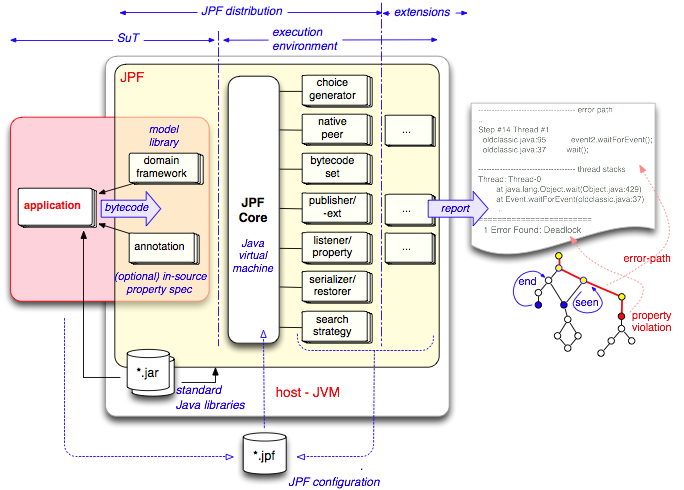
\includegraphics[height=5cm]{img/jpf-components}
\caption{\acrshort{acr:jpf} Workflow}
\label{fig:jpf:process}
\end{figure}

(A major design decision for JPF was to make it as modular and understandable to others as possible, but we sacrificed speed in the process—Spin is at least an order of magnitude faster than JPF.We believe this is a price worth paying in the long run.)

(Termination --- In order to ensure termination during explicit state model checking one must know when a state is revisited. It is common for a hashtable to be used to store states, which means an efficient hash function is required as well as fast state comparison.)

(States --- Specifically, each state consists of three components: information for each thread in the Java program, the static variables (in classes) and the dynamic variables (in objects) in the system. The information for each thread consists of a stack of frames, one for each method called, whereas the static and dynamic information consists of information about the locks for the classes/objects and the fields in the classes/object)

%(Explain the components/workflow, maybe)


%(Simple example) (Division by zero seems reasonable)
\begin{lstlisting}[
language=Java,
float,
caption={[Simple example with random values] The use of random values could lead to unexpected behavior. In this case, a division by zero could occur if certain combinations of random values are used.},
label=lst:jsp:random
]
import java.util.Random;

public class RandomExample {

  public static void main(String[] args) {
    Random random = new Random();
    int a = random.nextInt(2);
    int b = random.nextInt(3);
    int c = a/(b+a-2);
  }
}
\end{lstlisting}


(Features of JPF) (Explicit State, State Matching, Backtracking, Partial Order Reduction)

(Extension Points: Search strategies, Choice Generators, Listeners, Instruction Factories, Native Peers, Models, Publisher, consider presenting them as a list of concepts)

(Modules - Briefly mention them a an introduction to SPF)

\TUsubsection{Symbolic PathFinder (SPF)}
\label{subsec:spf}

(Definition of SPF)

(Explain its extension points: Choice Generators, Listeners, Symbolic Instruction Factory)

(Mention the solvers)







